% Based on a script by Stefano Rosatti
% author: Lukasz Kidzinski
% email: lukasz.kidzinski@stanford.edu
% Stanford University
% August 2016

% #########################################

\documentclass{beamer}
\usepackage{textpos}
\usepackage{graphicx}
\usepackage{amsmath}
\usepackage{amssymb}
\usepackage{booktabs}

\newcommand{\bT}{\mathbf{T}}
\newcommand{\cP}{\mathcal{P}}
\newcommand{\cS}{\mathcal{S}}
\newcommand{\vsmall}{\vskip 5px}
\newcommand{\vmedium}{\vskip 10px}
\newcommand{\vbig}{\vskip 20px}
\newcommand{\bA}{\mathbf{A}}
\graphicspath{ {img/} }
\usetheme{stanford}
\author[PIN-CHUN, HSU]{ Mingsheng Long$^{12}$, Yue Cao$^1$, Jianmin Wang$^1$, and Michael I. Jordan$^2$ }
\title[Deep Adaptation Networks]{\LARGE Learning Transferable Features with Deep
Adaptation Networks}
\date[May 17, 2017]{International Conference on Machine Learning, 2015}

\begin{document}

\setbeamercolor{itemize item}{fg=red}
\frame{\titlepage}

\begin{frame}[fragile]{Introduction}
\begin{itemize}
\item{Goal: enhance the transferability of features from task-specific layers}
\item{Proposed a Deep Adaptation Network DAN architecture}
  \begin{itemize}
    \item{general features can generalize well to a novel task; however, for specific features they cannot bridge the domain discrepancy}
  \end{itemize}

\item{some ways to enhance feature transferability}
  \begin{itemize}
    \item{by mean-embedding matching, feature transferability can be enhanced substantially}
    \item{utilizing multi-layer representations across domains in a reproducing kernel Hilbert space}
  \end{itemize}
\end{itemize}
\end{frame}

\begin{frame}[fragile]{Main Breakthrough}
\begin{itemize}
\item{\emph{generalizes deep CNN to the domain adaptation}}
\item{Deep adaptation of multiple task-specific layers, including output}
\item{Optimal adaptation using multiple kernel two-sample matching}
\end{itemize}
\end{frame}

\begin{frame}[fragile]{Deep Learning For Domain Adaptation}
\begin{itemize}
\item{None or very weak supervision in the \emph{target} task (new domain)}
  \begin{itemize}
  \item{Target classifier cannot be reliably trained due to over-fitting}
  \item{Fine-tuning is impossible as it requires substantial supervision}
  \end{itemize}
\item{Generalize related supervised source task to the target task}
  \begin{itemize}
  \item{Deep networks can learn transferable features for adaptation}
  \end{itemize}
\item{Hard to find big source task for learning deep features from scratch}
  \begin{itemize}
  \item{Transfer from deep networks pre-trained on unrelated big dataset}
  \item{Transferring features from distant tasks better than random features}
  \end{itemize}
\end{itemize}
\begin{figure}[h]
    \centering
    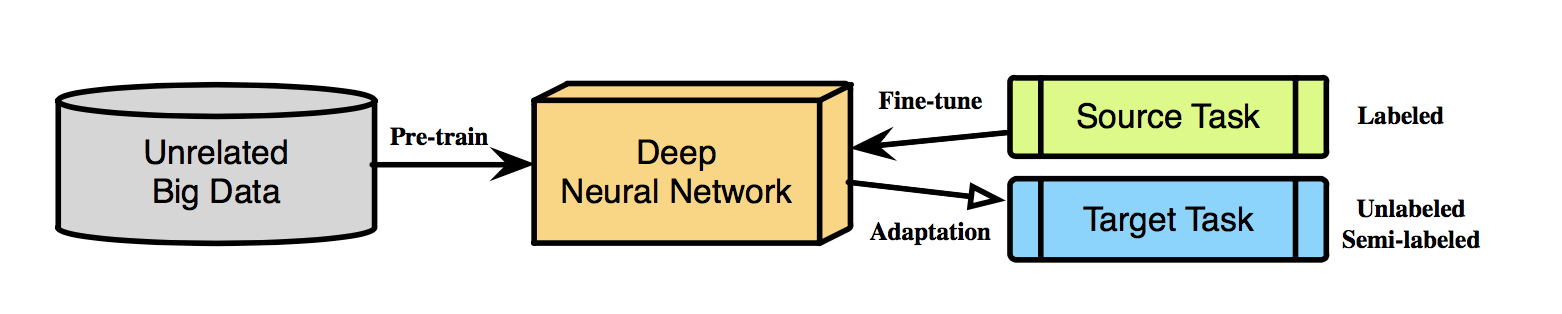
\includegraphics[width=1\textwidth]{fig1}
    \caption{\emph{Deep Learning for Domain Adaptation Workflow}}
    \label{fig:mesh2}
\end{figure}
\end{frame}

\begin{frame}[fragile]{How Transferable Are Deep Features?}
\begin{itemize}
  \item{Transferability is restricted by (Yosinski et al. 2014; Glorot et al. 2011)}
  \item{Specialization of higher layer neurons to original task (new task ↓)}
  \item{Disentangling of variations in higher layers enlarges task discrepancy}
  \item{Transferability of features decreases while task discrepancy increases}
\end{itemize}
\begin{figure}[h]
    \centering
    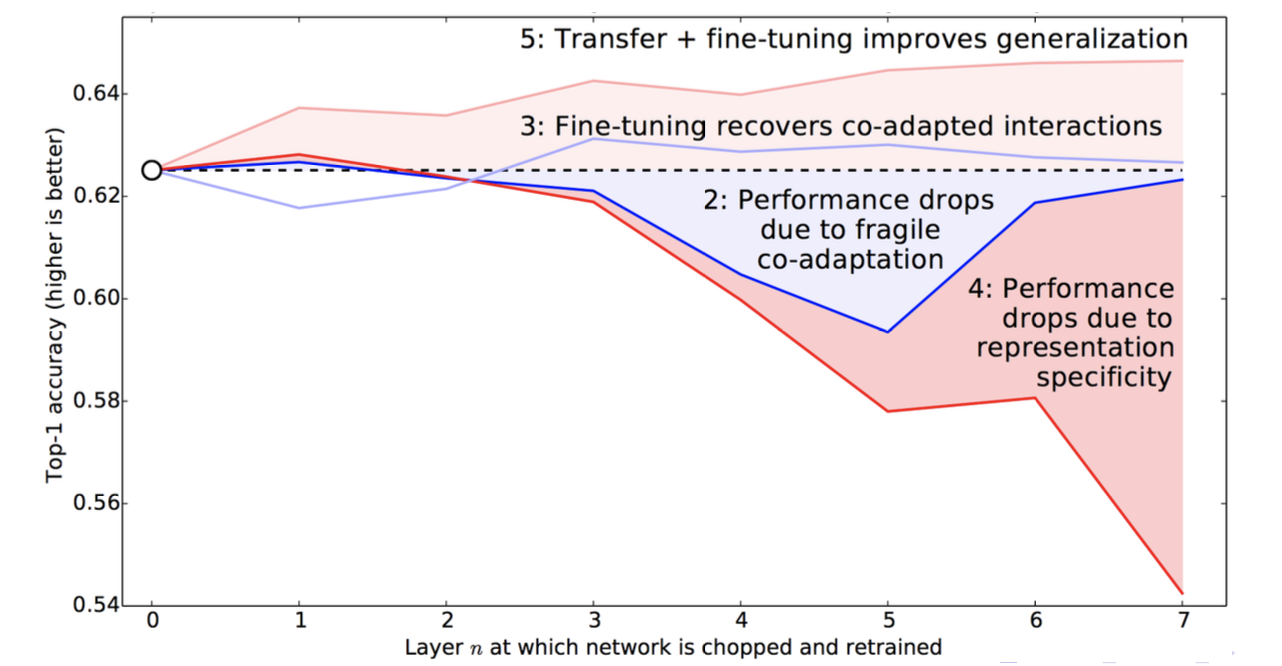
\includegraphics[width=0.5\textwidth]{fig2}
    \caption{\emph{Transferability of features decreases while task discrepancy increases}}
    \label{fig:mesh2}
\end{figure}
\end{frame}

\begin{frame}[fragile]{Deep Adaptation Network (DAN)}
\begin{block}{Key Observations (AlexNet) (Krizhevsky et al. 2012)}
\begin{itemize}
  \item{Comprised of five convolutional layers $conv1-conv5$ and three fully connected layers $fc6-fc8$}
  \item{Convolutional layers learn general features: safely transferable} 
  \begin{itemize}
  \item{Safely freeze $conv1-conv3$ \& fine tuned $conv4-conv5$}
  \end{itemize}
  \item{Fully-connected layers fit task specificicy: \emph{NOT} safely transferable} 
  \begin{itemize}
  \item{Deeply adapt $fc6-fc8$ using statistically optimal two-sample matching}
  \end{itemize}
\end{itemize}
\end{block}
\end{frame}


\end{document}
